\documentclass[parskip]{scrartcl}

\usepackage[margin=2.5cm]{geometry}
\usepackage{microtype}
\usepackage{abstract}
\usepackage[ngerman]{babel}
\usepackage{biblatex}
\addbibresource{quellen.bib}
\usepackage{csquotes}
\usepackage{hyperref}
\usepackage{graphicx}

% https://tex.stackexchange.com/a/313337
\usepackage{enumitem,amssymb}
\newlist{todolist}{itemize}{2}
\setlist[todolist]{label=$\square$}
\usepackage{pifont}
\newcommand{\cmark}{\ding{51}}%
\newcommand{\xmark}{\ding{55}}%
\newcommand{\todo}{$\square$}
\newcommand{\done}{\rlap{$\square$}{\raisebox{2pt}{\large\hspace{1pt}\cmark}}%
\hspace{-2.5pt}}
\newcommand{\wontfix}{\rlap{$\square$}{\large\hspace{1pt}\xmark}}

\setlist[itemize]{noitemsep}

\usepackage{tabularray}

\newcommand*{\eng}[1]{\textit{#1}}
\newcommand*{\feng}[1]{\eng{#1}}

\title{
    Analyse der Optimierungsverfahren mechanischer neuronaler Netzwerke \\ 
    \LARGE \normalfont Projektskizze
}
\author{Alexander Reimer \and Matteo Friedrich}
\date{\today}

\begin{document}
\maketitle

\tableofcontents

\begin{abstract}
    Wir wollen uns mit dem neuen, vergleichsweise wenig erforschtem Bereich der Mechanical Neural Networks, kurz MNNs, beschäftigen.
    Während die bisherige Forschung sich auf die technische, physische Implementation dieser Netzwerke fokussiert hat, wollen wir das Trainingsverfahren optimieren.
    Dazu wollen wir die bisher verwendeten Algorithmen (evolutionäres Lernen und Pattern Search) selbst implementieren und genauer sowie mit neuen Parametern ausprobieren und vergleichen.
    Außerdem wollen wir versuchen, eine Methode für Backpropagation bei MNNs zu entwickeln und implementieren, da eine solche unserer Recherche nach noch nicht ausprobiert wurde.

    Dafür werden wir uns jedoch auf die Anwendung dieser Algorithmen in einer Simulation beschränken. Die Ergebnisse sollten dennoch einen guten Startpunkt für reale MNNs bieten.

    Wir haben bereits eine Simulation sowie einen rudimentären evolutionären Algorithmus umgesetzt.
\end{abstract}

\section{Einleitung}

Inspiration für dieses Projekt ist ein Artikel von 2022 mit dem Titel \enquote{Mechanical neural networks: Architected materials that learn behaviors} \cite{Lee2022}.

Es ist der erste veröffentlichte Artikel, der sogenannte \feng{mechanical neural networks}, kurz MNNs, beschreibt, ein neuer Forschungsbereich, in dem neuronale Netzwerke in der physischen Welt umgesetzt werden.
Dazu werden Knotenpunkte gebaut, welche mit Federn mit variabler Steifigkeit verbunden werden.

MNNs können aufgrund der variablen Steifheit der Federn als lernfähiges Material verwendet werden, welches seinen Bedingungen oder gewünschten Verwendungszwecken angepasst werden kann.

Dazu kann das Material sowohl in einer Simulation als auch physisch, durch Sensoren in den Federn, trainiert werden.

\begin{figure}
    \centering
    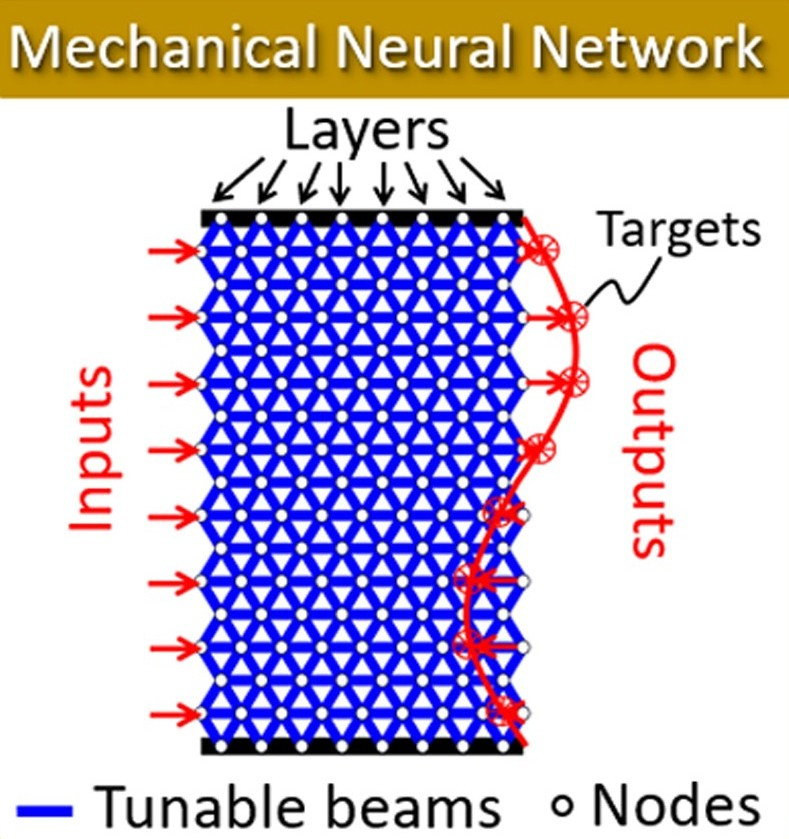
\includegraphics[width=0.4\linewidth]{bilder/mnn1-1.jpg}
    \label{fig:mnn1-1}
    \caption{Repräsentation eines MNN (von \cite{Lee2022})}
\end{figure}

\begin{figure}
    \centering
    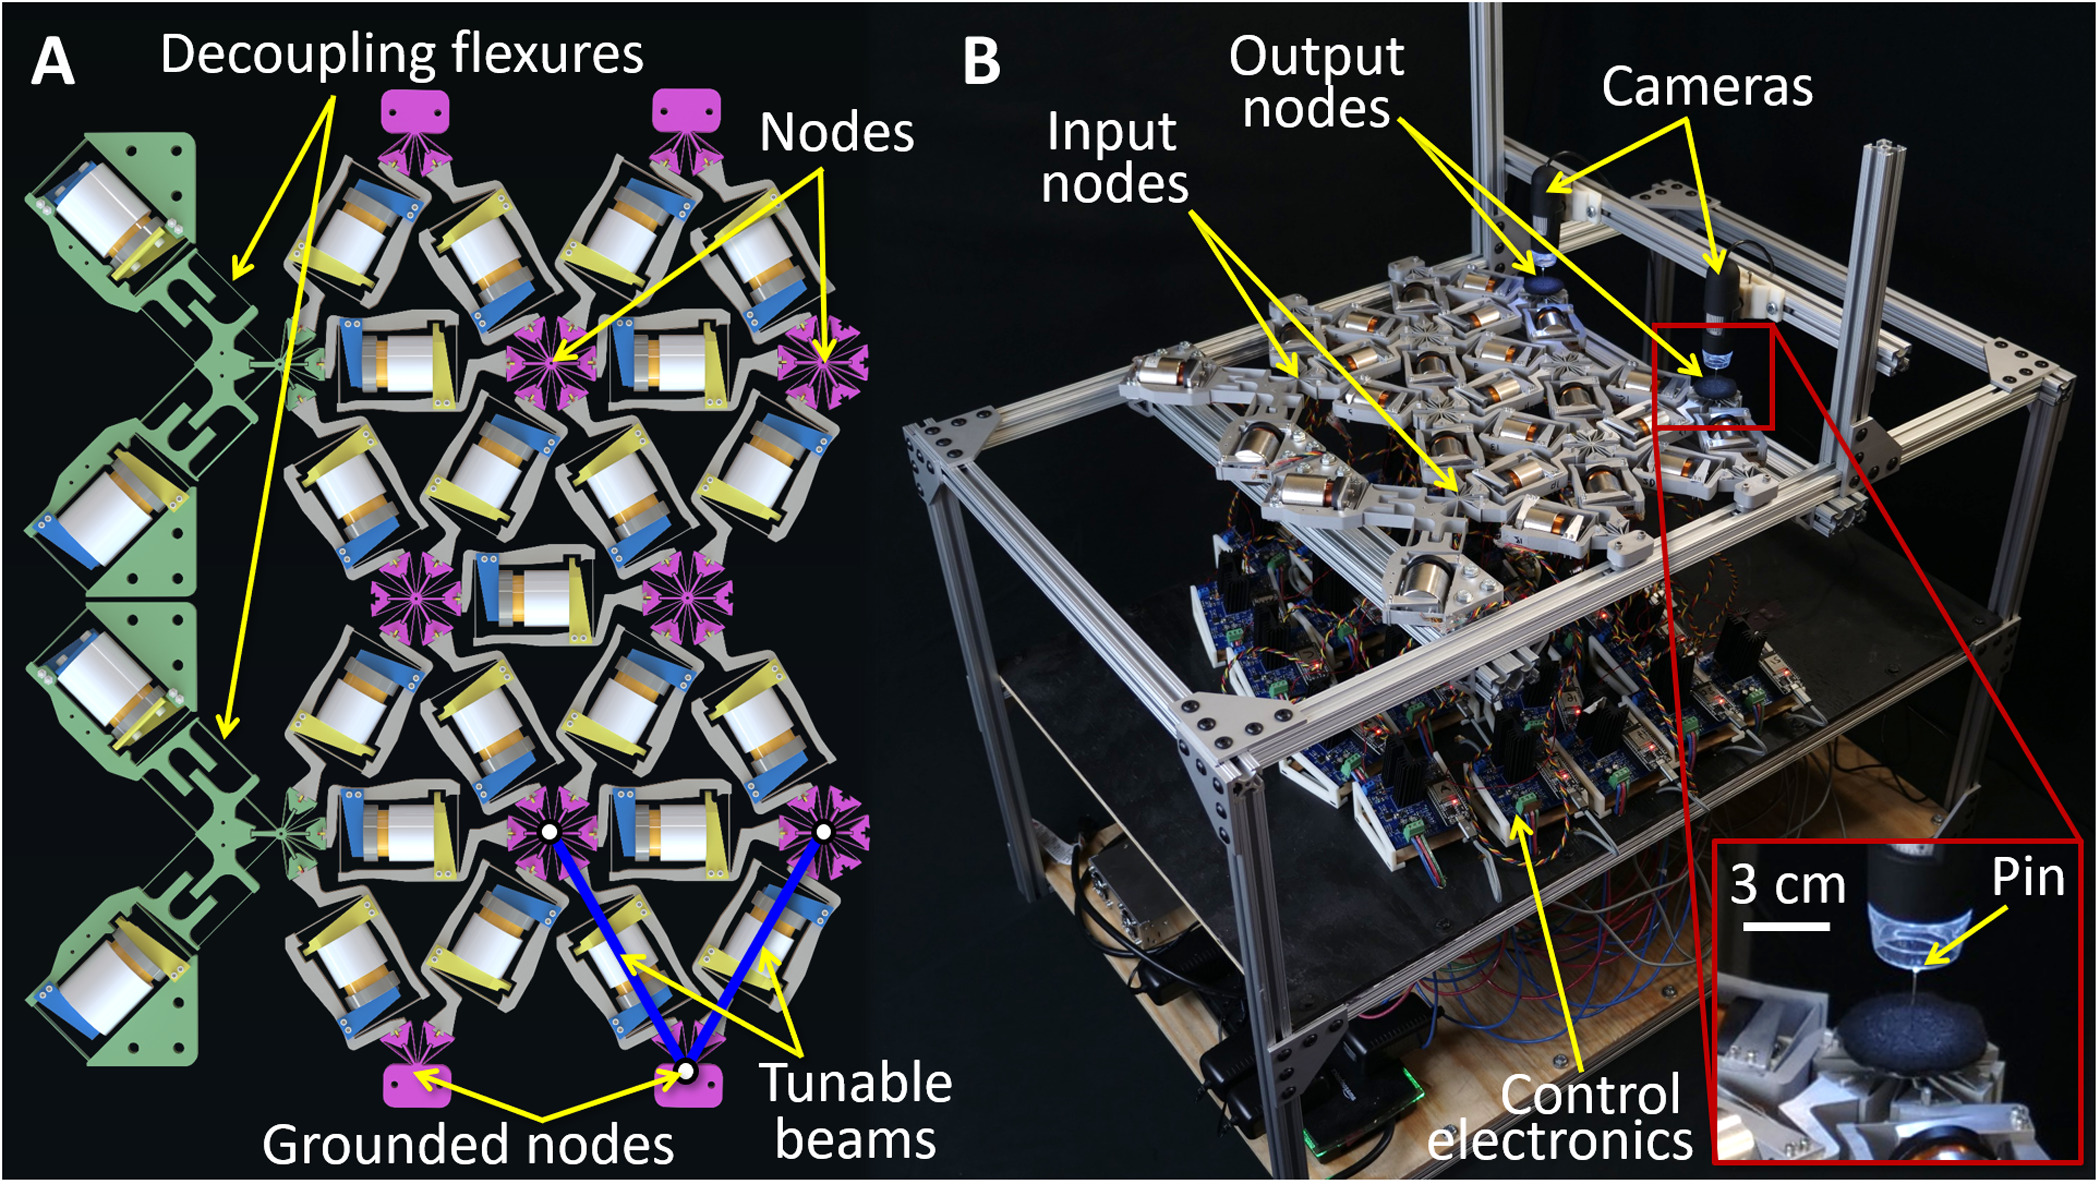
\includegraphics[width=0.7\linewidth]{bilder/mnn2-1.jpg}
    \label{fig:mnn2-1}
    \caption{Mechanische Umsetzung eines MNN (von \cite{Lee2022})}
\end{figure}

\section{Forscherfrage}

Ziel des Projektes ist es, ein neues Optimierungsverfahren für das Trainieren von MNNs zu entwickeln, sowie dieses mit den beiden im Artikel verwendeten Verfahren -- ein evolutionärer Algorithmus und Pattern Search -- zu vergleichen.

Ziel des Projektes ist es nicht, ein MNN selbst mechanisch umzusetzen.
Es wird davon ausgegangen, dass 
\begin{enumerate}
    \item ein Vergleich der Verfahren in einer Simulation auch für das physische Trainieren der mechanischen Netzwerke aussagekräftig sein könnte und
    \item ein \enquote{Vortrainieren} eines physischen MNN mit einer Simulation die Gesamtzeit zum Trainieren verkürzt und somit Optimierungsverfahren, auch wenn sie nur in einer Simulation verwendet werden, von Nutzen sind.
\end{enumerate}

\section{Zeitplan}

\begin{tblr}{hlines, vlines, colspec={Q[c, 0.3cm] Q[r, 2.7cm] X l}, width=\textwidth}
    % Status
    & Zeit & Thema & Person \\
    \hline
    \done & & Proof-of-Concept für MNNs & Matteo \\
    \done & & Refactor des ersten Proof-of-Concept & Alex \\
    \done & & Proof-of-Concept für analytische Umsetzung der Simulation & Matteo \\
    \done & & Umsetzung des Trainierens mehrerer Verhaltensweisen gleichzeitig & Alex \\
    \done & \textbf{bis 30.11.2023} & JuFo-Anmeldung \\
    \todo & & Projektskizze anfertigen & Alex \\
    \todo & bis 3.12.2023 & weitere Literatur lesen (\cite{Hopkins2023, Zadpoor2023, Napolitano2022}) & Alex \\
    \todo & bis 3.12.2023 & Implementierung analytischer Definition für Simulation (Proof-of-Concept) im Hauptprojekt & Matteo \\
    \todo & bis 10.12.2023 & Proof-of-Concept für Gradient Descent & \\
    \todo & bis 10.12.2023 & Oberflächliche Recherche zu Pattern Search: Leicht umzusetzen? Wenn nein, dann erstmal außen vor lassen (\cite{Lee2022} hat bereits gezeigt, dass schlechter als evolutionär, auch wenn mit stark unterschiedlicher Trainingsdauer) & \\
    \todo & bis 17.12.2023 & Verbesserung evolutionärer Algorithmus & \\
    & & Projektskizze aktuell halten & Alex \\
    \todo & & UML-Diagramm des Codes & Alex \\
    \todo & & Recherche zu Resonanzfrequenzen: wirklich ein Problem? Wenn ja, Resonanzfrequenzen in Simulation analysieren (FFT?) & \\
    \todo & \textbf{15.01.2023} & Abgabe Bericht & \\

\end{tblr}

\section{Materialien}

\begin{itemize}
    \item Laptop (i7-11800H, 16\,GB, RTX 3060)
    \item Julia
    \begin{itemize}
        \item DifferentialEquations.jl und LinearAlgebra.jl für analytische Definition der Simulation des Federsystems
        \item Graphs und MetaGraphsNext für Modellierung des Netzwerks als Graph
        \item GLMakie und Observables für Visualisierung
    \end{itemize}
\end{itemize}

\section{Erwartete Schwierigkeiten}

\begin{itemize}
    \item 
\end{itemize}

\section{Bisherige Ergebnisse}

Quellcode: Siehe GitHub-Repository \cite{RepoMNN}.
Siehe Abb. \ref{fig:uml} für ein UML-Diagramm des Projekts.

\begin{figure}
    \centering
    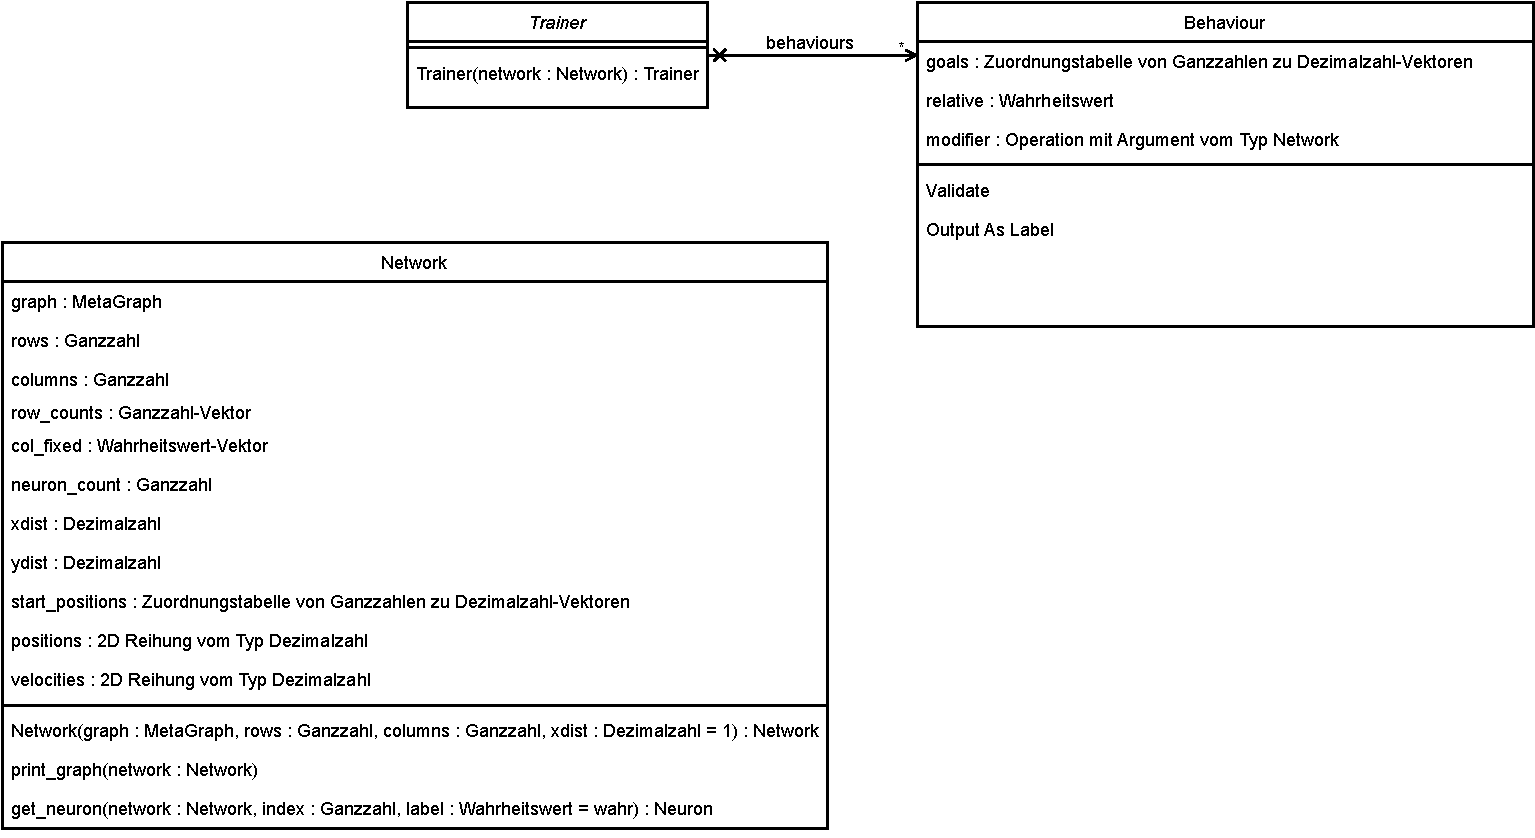
\includegraphics[width=0.9\textwidth]{bilder/uml.pdf}
    \caption{UML-Diagramm des Programm-Aufbaus.}
    \label{fig:uml}
\end{figure}

Wie teilweise auch aus dem Zeitplan ersichtlich wurden bereits die Simulation, eine Optimierung dieser durch eine analytische Funktion, die Visualisierung und Animation des Netzwerks sowie ein simpler evolutionärer Algorithmus implementiert.

Trainieren mit diesem evolutionären Algorithmus hat bereits bei einzelnen, simplen Verhaltensweisen Erfolg gezeigt.

Bereits probierte und erfolgreich antrainierte Verhaltensweisen:

\begin{itemize}
    \item Links eine Kraft nach rechts ausüben; Bewegung der Ausgangsneuronen nach rechts 
    \item Links eine Kraft nach rechts ausüben; Bewegung der Ausgangsneuronen nach links
    \item Links eine Kraft nach links ausüben; Bewegung der Ausgangsneuronen nach rechts
\end{itemize}

\section{Gruppe}

Da es sich um Grundlagenforschung handelt, ist viel Recherche sowie Trial-and-Error nötig; es gibt keine fertige Anleitung.
Deshalb arbeiten wir zusammen daran.

Aufgaben werden aufgeteilt, jedoch gibt es keine übergreifende Zuständigkeitsbereiche. Wir arbeiten beide an Programmierung, Recherche und Dokumentation.

\section{Externe Kooperationspartner}

Es gibt keine externe Kooperationspartner.

\section{Literatur}

\printbibliography

\end{document}